Genetic programming is a branch of artificial intelligence inspired by biological evolution. It is a machine learning
technique that optimizes a population of computer programs until they start performing the user specified
functionality. Like the more widespread genetic algorithms (GA), genetic programming uses an evolutionary algorithm
based methodology to iterate through solutions until a correct one is found. In genetic programming a 
predefined size \textbf{population} is iterated through a user defined number of \textbf{generations}. 
The population consists of \textbf{individuals} which are programs represented as a tree structure.
This tree structure is constructed from a pre-defined set of \textbf{primitives} and \textbf{terminals}.
The primitives represent the functions from which the individual is constructed and
the terminals represent the bottom nodes of the tree, they can be both arguments and constants. A tree representation of an individual
can be seen in figure \ref{fig:ind}
\begin{figure}[htp]
\centering
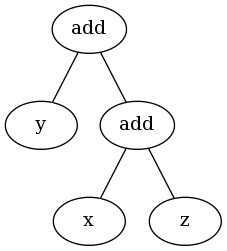
\includegraphics[scale=0.6]{Figures/ind.png}
\caption{An example of a genetic programming individual that represents x+y+z}
\label{fig:ind}
\end{figure}
A genetic program needs a \textbf{fitness function} through which each individual
is evaluated and compared. This way the correctness of the program can be calculated. Usually there are two type of fitness function 
minimum and maximum where minimum is looking for individuals with fitness values closer to 0 (where 0 usually means that a solution is found)
and maximum for the individuals with highest fitness result.
\paragraph{}
Genetic program randomly generates individuals for the first generation, evaluates them through the 
fitness function and creates new programs through \textbf{crossover} and \textbf{mutation}. Crossover 
is used to combine the genetic information of two individuals which means switching the nodes of a tree of one individual
with another as seen in figure \ref{fig:cross}. With a tree-based representation replacing a node means replacing the whole branch. When mutation
is applied to an individual a single node is replaced with a new randomly generated one. Changing a single
node can mean changing the whole branch shown in figure \ref{fig:mut}. After crossover and mutation are applied to the population a new generation
that consists of the children, individuals from the old population and mutated individuals is created
hence the iterations continue until the generations are completed. A result may not be found in the end of the generations.
The result of a genetic program is a heuristic, a stochastic method - no guarantee of success.
\begin{figure}[htp]
\centering
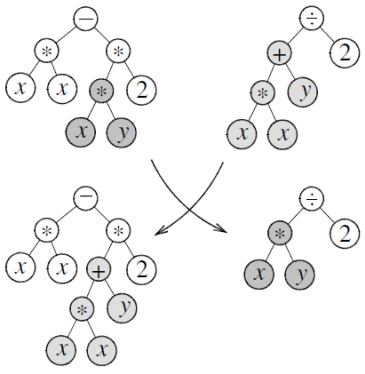
\includegraphics[scale=0.8]{Figures/crossover.png}
\caption{An example of a crossover between two individuals and their children as result}
\label{fig:cross}
\end{figure}

\begin{figure}[htp]
\centering
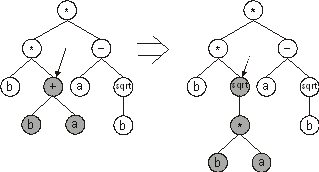
\includegraphics[scale=1.2]{Figures/mutation.png}
\caption{An example of a mutation applied to an individual}
\label{fig:mut}
\end{figure}

One of the problems with genetic programming is searching for the correct parameters to solve a specific problem. For each problem
a specified number of populations, generations needs to be provided e.g the percentage of the population to which crossover and
mutation are going to be applied. In more advanced cases the types of mutation and crossover algorithms need
to be specified. Another complication is choosing the correct fitness function to evaluate the correctness of the individuals. If 
an incorrect fitness function is defined an individual with seemingly good fitness value may be far from correct. The primitive
and terminal sets need to be wisely chosen as well. If too many primitives are chosen the generations might not be enough to 
find a solution to the problem because the search boundaries were expanded. However if small sets are chosen we are 
limiting the search boundaries or the individuals won't have a sufficient primitive set to satisfy the required functionality.
\paragraph{}
Using this methodology multiple problems can be solved. A common and a simple one is symbolic regression. In the case
of symbolic regression an individual represents a mathematical expression and is evaluated against another expression
specified in the fitness function. In this project this technique is uesed as a proof
of concept for the capabilities of the framework.